\chapter{Definitionen}
\label{ch:chapter02}
Dieses Kapitel erklärt und beschreibt einige der zentralen Begriffe zum Thema des Hosts und der Berechtigungsstrukturen.
Dadurch soll der Leser ein Grundverständnis erhalten, um die folgenden Kapitel zu verstehen.

%
% Section: Der erste Abschnitt
%

\section{Host/Mainframe}
\label{sec:Host}
Der Host bzw. Mainframe ist ein Komplex aus verschiedenen Hochleistungscomputern.
Der Anbieter "`IBM"' definiert diesen dabei wie folgt: 
\newline
\newline
\textit{"`At their core, mainframes are high-performance computers with large amounts of memory and processors that process billions of simple calculations and transactions in real time."'} \cite{Mainframe}
\newline
\newline
Oder übersetzt:
\newline
\newline
\textit{"`Im Kern besteht der Mainframe aus Hochleistungsrechnern, welche über einen großen Speicher verfügen, und in der Lage sind, Milliarden von einfachen Prozessen und Transaktion in Echtzeit durchzuführen."'} \cite{Mainframe}
\newline
\newline
Dabei spielt der Mainframe eine wichtige Rolle in der Finanzindustrie, welche widerstandsfähige, sichere und agile Server benötigt.
Dies ist der Fall, weil die Finanzindustrie über viele sensible Daten verfügt.
Daher müssen die Server sicher und widerstandsfähig sein, damit diese Daten nicht verloren gehen oder gestohlen werden.
Zudem müssen die Server agil sein, da sich die Technologie und die Regulierungen für den Mainframe sich stetig ändern und dieser daher immer auf dem neuesten Stand sein muss.
Der Mainframe muss die Regularien der \ac{VAIT} erfüllen, die von der \ac{BaFin} aufgestellt werden.
Die \ac{BaFin} soll eine konsistente IT-Strategie vorgeben, an die sich die Unternehmen halten müssen. \cite{Vait}

\section{Berechtigung}
\label{sec:Berechtigung}
Dabei definiert die \ac{NIST}, welche eine Institut der amerikanischen Regierung ist, Berechtigungen wie folgt:
\newline
\newline
\textit{"`The right or a permission that is granted to a system entity to access a system resource."'} \cite{Auth}
\newline
\newline
Dies bedeutet:
\newline
\newline
\textit{"`Das Recht oder die Erlaubnis haben, um auf System Ressourcen einer Systemeinheit zu zugreifen."'} \cite{Mainframe}
\newline
\newline
Im Kontext des Mainframebereiches betrifft dies bei Helvetia hauptsächlich das Betrachten und Zugreifen über Dialogmasken auf Daten.
\begin{figure}[h!]
 \centering
 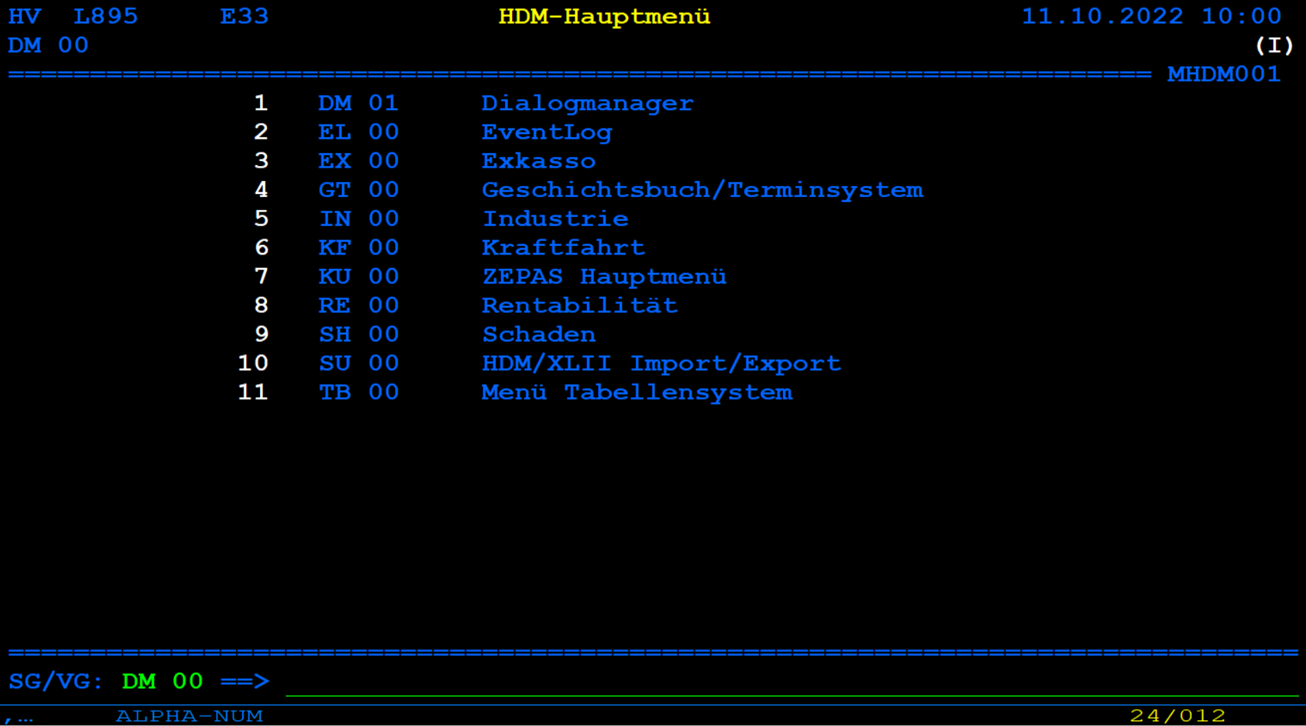
\includegraphics[width=1\textwidth]{gfx/Picture/Dialog.PNG}
 \caption{Beispiel Dialogmaske}
 \label{fig:Dial}
\end{figure}
Die Grafik (\ref{fig:Dial}) zeigt eine solche Dialogmaske.
Anhand dieser Dialogmaske kann man erkennen, dass der Nutzer USER$895$ für die aufgezählten weiteren Dialogmasken (EL$00$, EX$00$, ...) zumindest die Leseberechtigung hat, da diese auf der Dialogmaske DM$00$ angezeigt werden.
Zudem hat dieser die Schreibberechtigungen auf die Dialogmaske DM$00$, da dieser sich in dieser Maske aufhält. 
\newline
\newline
\begin{figure}[h!]
 \centering
 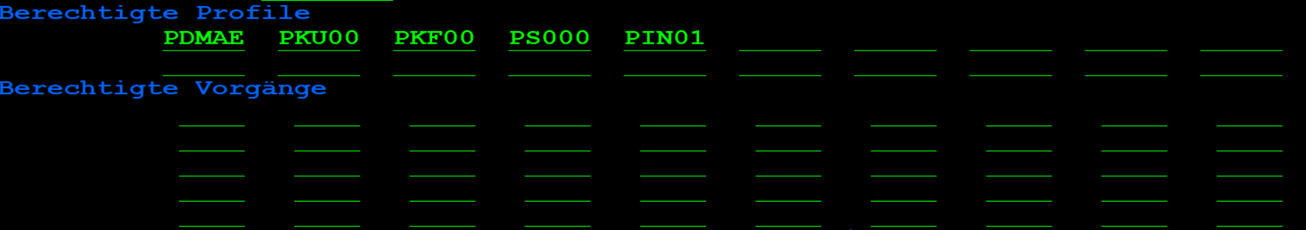
\includegraphics[width=1\textwidth]{gfx/Picture/Berechtigung.PNG}
 \caption{Berechtigungsdialogmaske}
 \label{fig:Berch}
\end{figure}
In dieser Grafik (\ref{fig:Berch}) kann man die Profile und individuellen Berechtigungen sehen, die der Nutzer USER$895$ besitzt.
Dabei sind Profile eine Ansammlung von Berechtigungen.

\section{Berechtigungsstruktur}
\label{sec:Berechtigungsstruktur}
Eine Berechtigungsstruktur besteht aus den Berechtigungen, die im Unterkapitel (\ref{sec:Berechtigung}) definiert werden, sowie aus einer Struktur.
Dabei definiert Oxford den Begriff Struktur wie folgt:
\newline
\newline
\textit{"`the way in which the parts of something are connected together, arranged or organized; a particular arrangement of parts"'} \cite{Struct}
\newline
\newline
Dies bedeutet, dass die Teile miteinander verknüpft, angeordnet oder organisiert sind. \cite{Struct}
\newline
In diesem Zusammenhang meint der Begriff Berechtigungsstruktur die Verknüpfung, Anordnung oder Organisation von Berechtigungen.
\begin{figure}[h!]
 \centering
 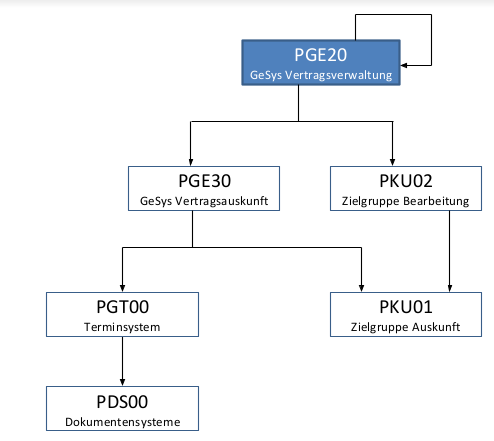
\includegraphics[width=1\textwidth]{gfx/Picture/Struktur.PNG}
 \caption{Teilausschnitt der Berechtigungsstruktur der Helvetia}
 \label{fig:Teil}
\end{figure}
Wie man in der Grafik (\ref{fig:Teil}) erkennen kann, sind die Profile hierarchisch aufgebaut.
Diese Profile beinhalten die Berechtigungen.
\begin{figure}[h!]
\hspace*{-4cm}
 \centering
 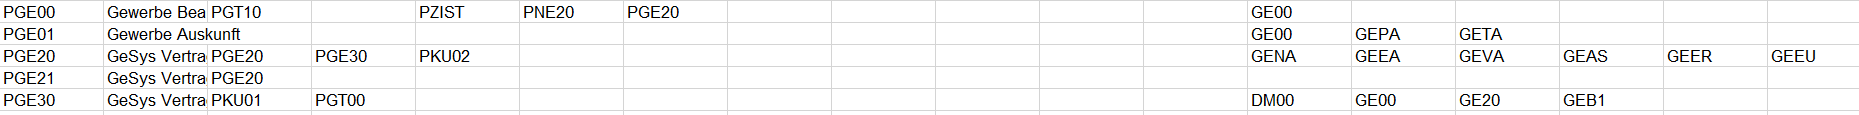
\includegraphics[width=1.6\textwidth]{gfx/Picture/Ber.PNG}
 \caption{Berechtigungen für die Profile PGE$20$ und PGE$30$}
 \label{fig:Ber}
\end{figure}
\newpage
Die Grafik (\ref{fig:Ber}) zeigt, dass die Profile PGE$20$ und PGE$30$ zum Beispiel über die folgenden Berechtigungen verfügen:
\begin{itemize}
	\item DM$00$
	\item GEEA
	\item GEVA
	\item GE$20$
\end{itemize}
Daher ist die aktuelle Berechtigungsstruktur bei der Helvetia hierarchisch.

\section{IAM}
\label{subsec:IAM}
Die Virginia IT Agency beschreibt IAM wie folgt: \textit{"`Identity management is the capability to manage all user accounts and profiles that can be identified with each person across the IT environment via user roles and business rules. Access management is the ability to manage access control policies across multiple platforms. (...) An integral part of identity management is to ensure that users have secure, convenient access to the resources needed (and only the resources needed) to perform their work."'} \cite{Virg07} (S.3)
\newline
\newline
Oder übersetzt:
\newline
\newline
Das \ac{IAM} ist eine Möglichkeit, sämtliche Nutzer und Profile, welche man zu den jeweiligen Personen über die IT-Umgebung über Nutzerrollen und Businessregeln zu ordnen kann, zu handhaben. Dabei ist die Zugriffverwaltung die Möglichkeit die Zugriffskontrolle über Regeln auf verschiedenen Plattformen einzuhalten. Ein wichtiger Teil von \ac{IAM} ist sicherzustellen, dass die Nutzer einen sicheren Zugriff auf die Ressourcen haben und auch nur auf die Ressourcen, die sie benötigen, um ihre Arbeit zu erledigen. \cite{Virg07} (S.3)
\begin{figure}[h!]
 \centering
 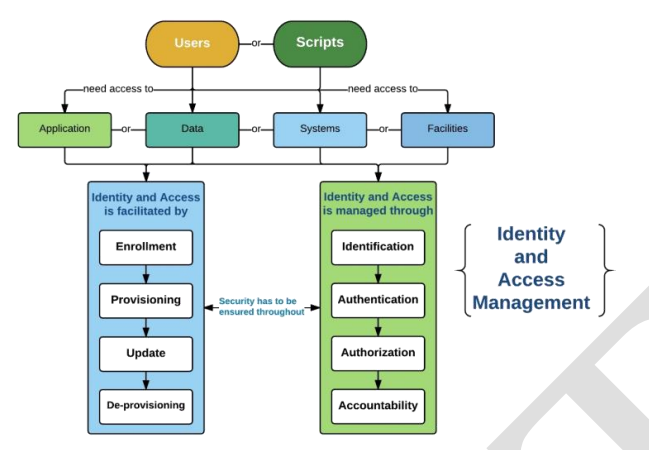
\includegraphics[width=1\textwidth]{gfx/Picture/IAM.PNG}
 \caption{Übersicht von IAM \cite{Moha19}}
 \label{fig:IAM}
\end{figure}
\newpage
Im Bild (\ref{fig:IAM}) kann man erkennen, dass, wenn ein Nutzer oder Programm Zugriff auf eine Ressource möchte, dieser die Identifizierung, Authentifizierung, Autorisierung, sowie Rechtschaffenheit vorlegen und einhalten muss. \cite{Moha19}
Wenn der Nutzer Lucas Stumm beispielsweise auf Daten des Hosts zugreifen möchte, muss dieser durch verschiedene Schritte gehen.
Als Erstes muss sich dieser mittels Nutzernamens und Passworts identifizieren.
Während dieser sich durch die Menüs manövriert , wird überprüft, ob Lucas Stumm überhaupt die Berechtigungen hat, diese Menüs sehen und auswählen zu können.
Wenn dies der Fall ist, kann der Nutzer auf die Daten zugreifen.
\newline
Im Rahmen dieser Ausarbeitung handelt es sich bei den Ressourcen um die Berechtigungen (\ref{sec:Berechtigung}).
